
\chapter{An Overview of \emph{Ravel}}

\label{tutorial}

\section{Slicing, Dicing and Rotating Data}

A Ravel is a graphical representation of multi-dimensional data. Unlike
a spreadsheet, which has only two dimensions, a Ravel can have as
many dimensions as your data. You manipulate the axes of a Ravel to
select the components of your data that you wish to see, and those
components are then the output of the Ravel, which can be graphed
or displayed directly, or attached to variables which can be further
analysed using the flowchart equation capabilities of \emph{Ravel}.
The Ravel below loads data from the \htmladdnormallink{\emph{Bank of International Settlements}}{https://data.bis.org/bulkdownload}
on house prices. This data has four dimensions:
\begin{description}
\item[Date] Quarterly data from 1927 till 2024: 388 entries 
\item[Unit of Measure] House Price Index where 2010 = 100; 2 entries 
\item[Value] Nominal or Real (CPI-deflated) prices: 2 entries 
\item[Reference Area] Country or Region: 62 entries 
\end{description}
\newpage

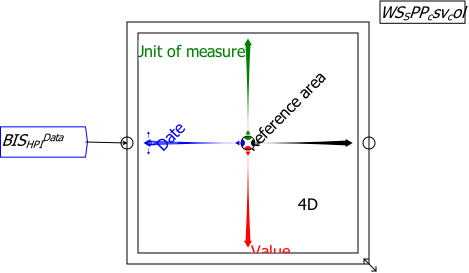
\includegraphics{images/tut00Ravel}

When a Ravel is first attached to data, it outputs the entire data
set---which is indicated by the dimension count \emph{4D} in the
lower right quadrant of this Ravel. You can see this by attaching
a Sheet to the output port of the Ravel:

\noindent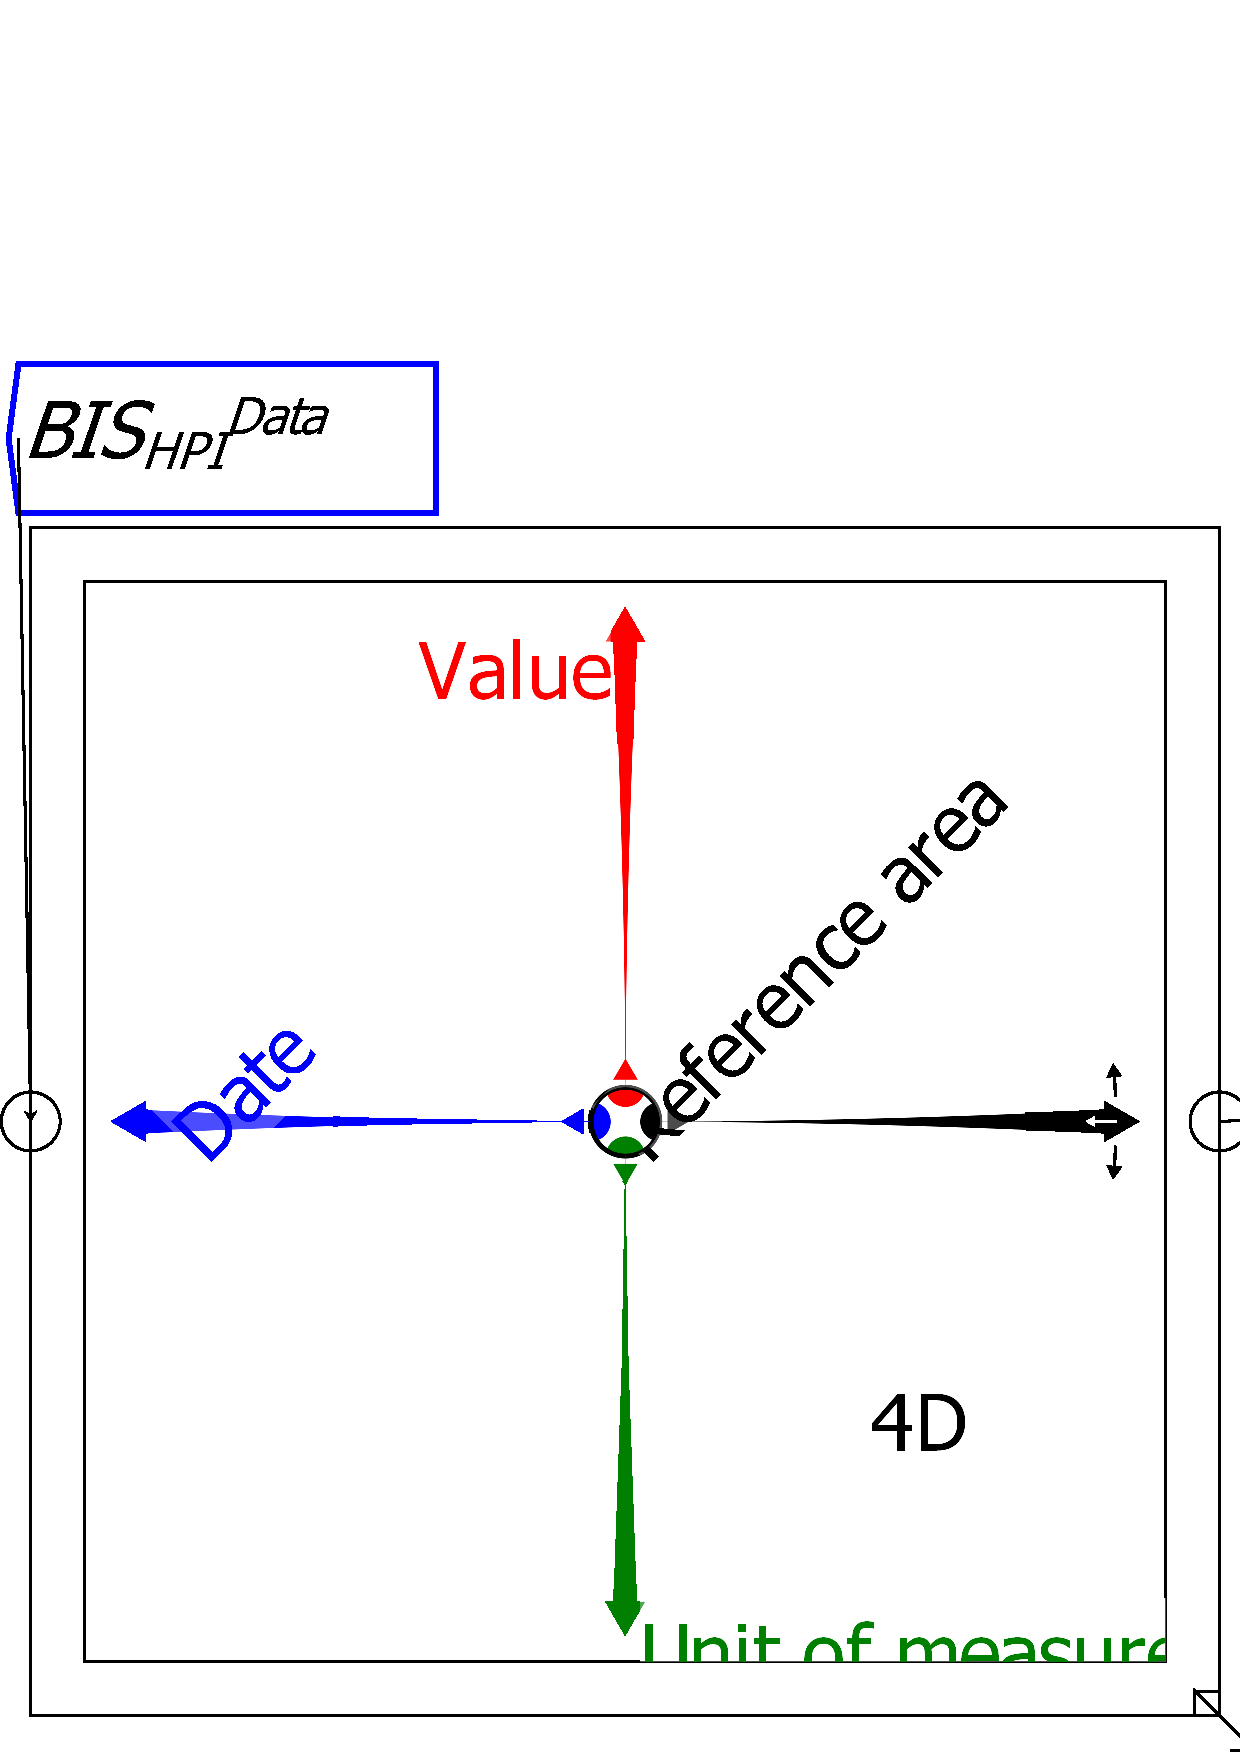
\includegraphics[width=\textwidth]{images/tut01Ravel4DwithSheet}

The right-pointing axis of the Ravel determines what is shown on the
rows of the sheet, while the down-pointing Axes of the Ravel determine
what is shown by the columns. At present these are Reference Area
by Value, and the sheet shows a slice of that data for the first entry
in the Date and Value axes--1927-Q3, and Nominal (unadjusted for
inflation).

It would be more useful to see the data by Reference Area by Date.
To get that view, click the left mouse button on the arrowhead of
the Date axis, hold the button down, and rotate the axis into the
down direction, which is currently occupied by the Value axis. When
you release the mouse button, the Date axis will replace the Unit
of measure axis in the down direction, and the data in the Sheet will
now have countries by rows and Quarters by columns.

\noindent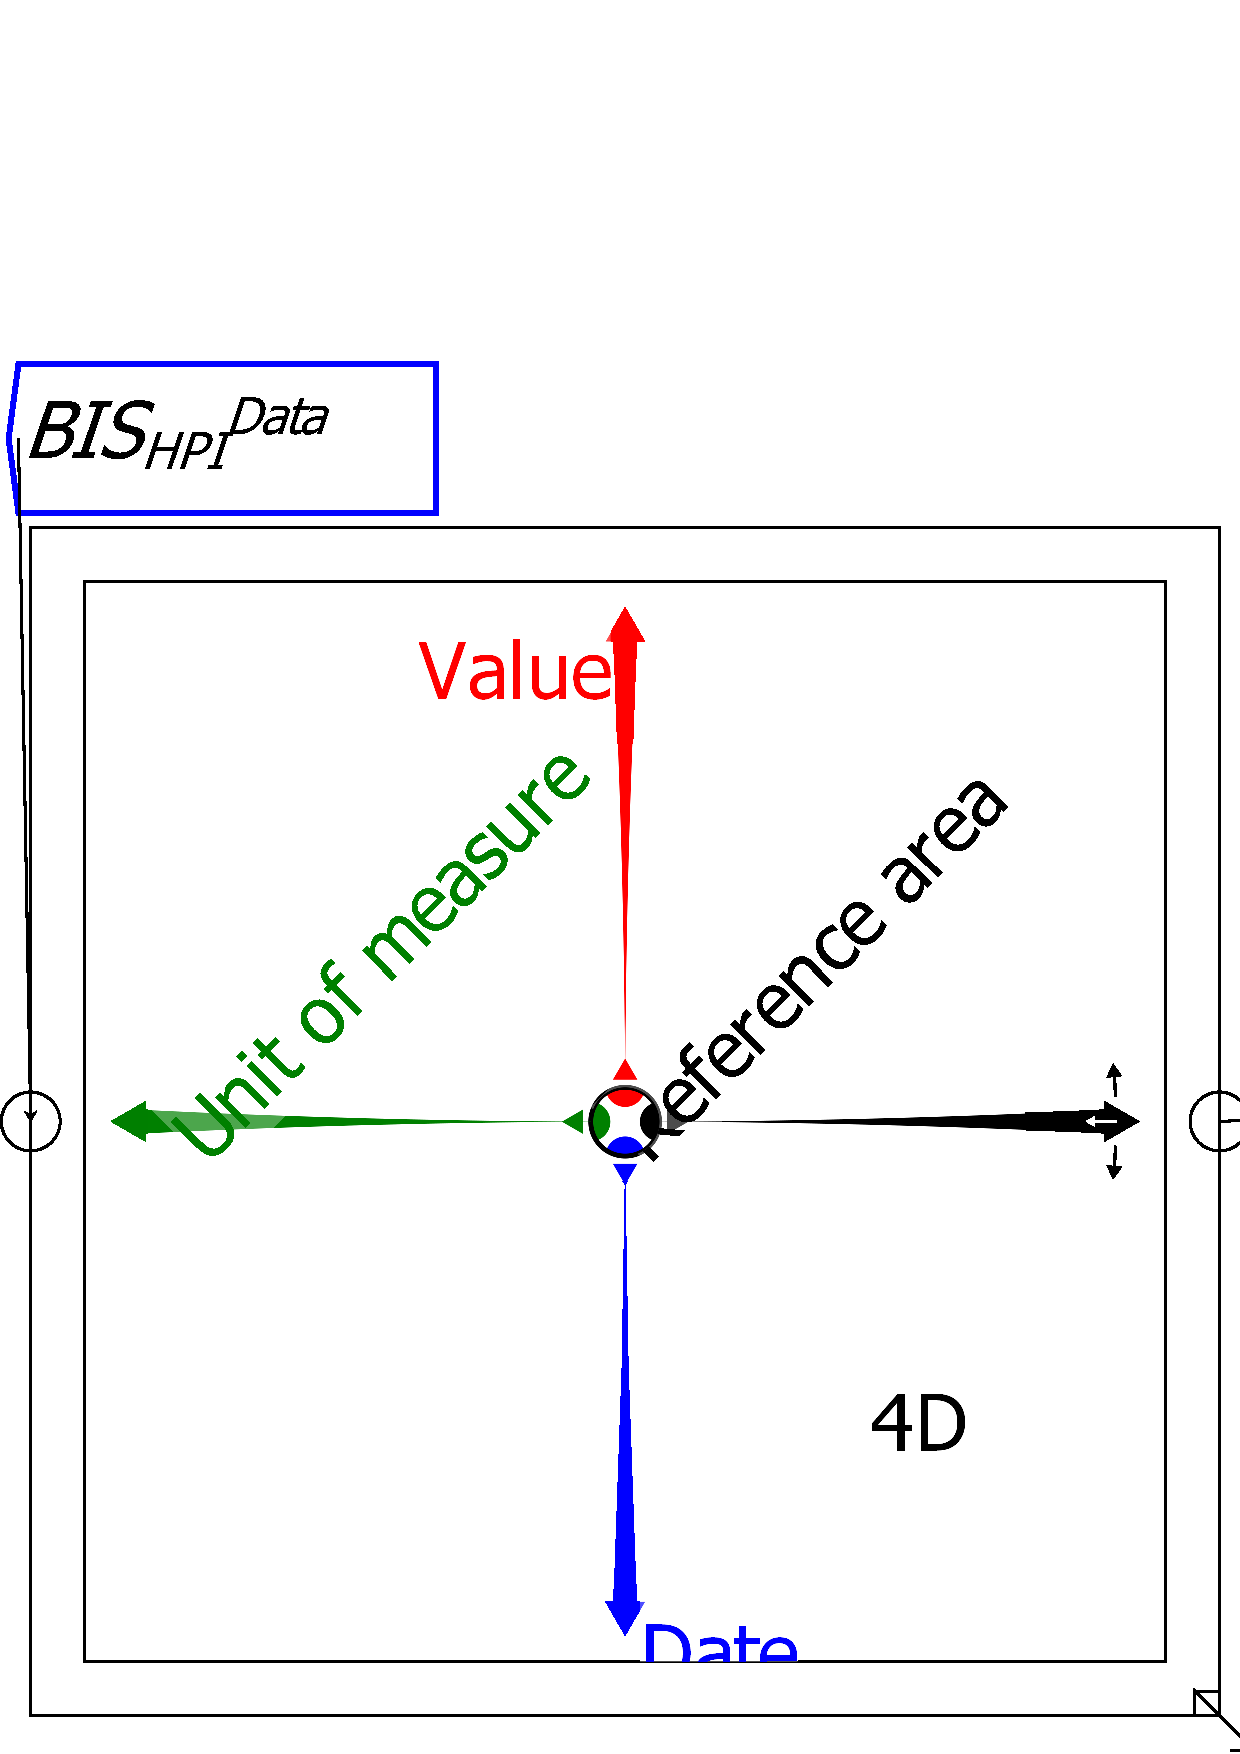
\includegraphics[width=\textwidth]{images/tut02HPI4DwithSheetRotatedCountryDate}

The Sheet is still blank, because there is no data for the current
selections--there is no data for Index for Nominal House Prices in
the very first Quarters of the data (in the years 1927 and 1928) for
the first countries in the file in alphabetical order.

To see data immediately, you can take advantage of a feature of the
Sheet: it can display the first few rows and columns of data (the
default setting), which we call the Head, the last few (the Tail),
or a few of both (Head and Tail). To show the last few rows and columns,
right-click on the Sheet and choose Row Slices/Tail and Column Slices/Tail".
That will then show you the last countries in the data file in alphabetical
order, and the last quarters in the data file.

The data still shows the Nominal Index data, since these are the first
entries in the other two axes. You can control the entry shown using
the selector dots on those two axes: these are the coloured dots that
are currently within the inner circle of the Ravel. Selector dots
can be moved:
\begin{itemize}
\item By using the mouse. Click on a dot and drag it to the required selection;
or 
\item By using the arrow keys. Use the mouse to move the cursor so that
it is hovering over an axis; then use the up or right arrow key to
move the dot out towards the arrowhead on an axis, or the down or
left arrow key to move back towards the center. 
\end{itemize}
To see the Real (CPI-adjusted) annual rate of change of house prices,
use the selector dot on those two axes. That selection is shown below--where
Date has also been rotated to the rows so that Countries are shown
by the columns. This already gives one interesting insight: house
prices were on average falling across advanced countries in 2023.

\noindent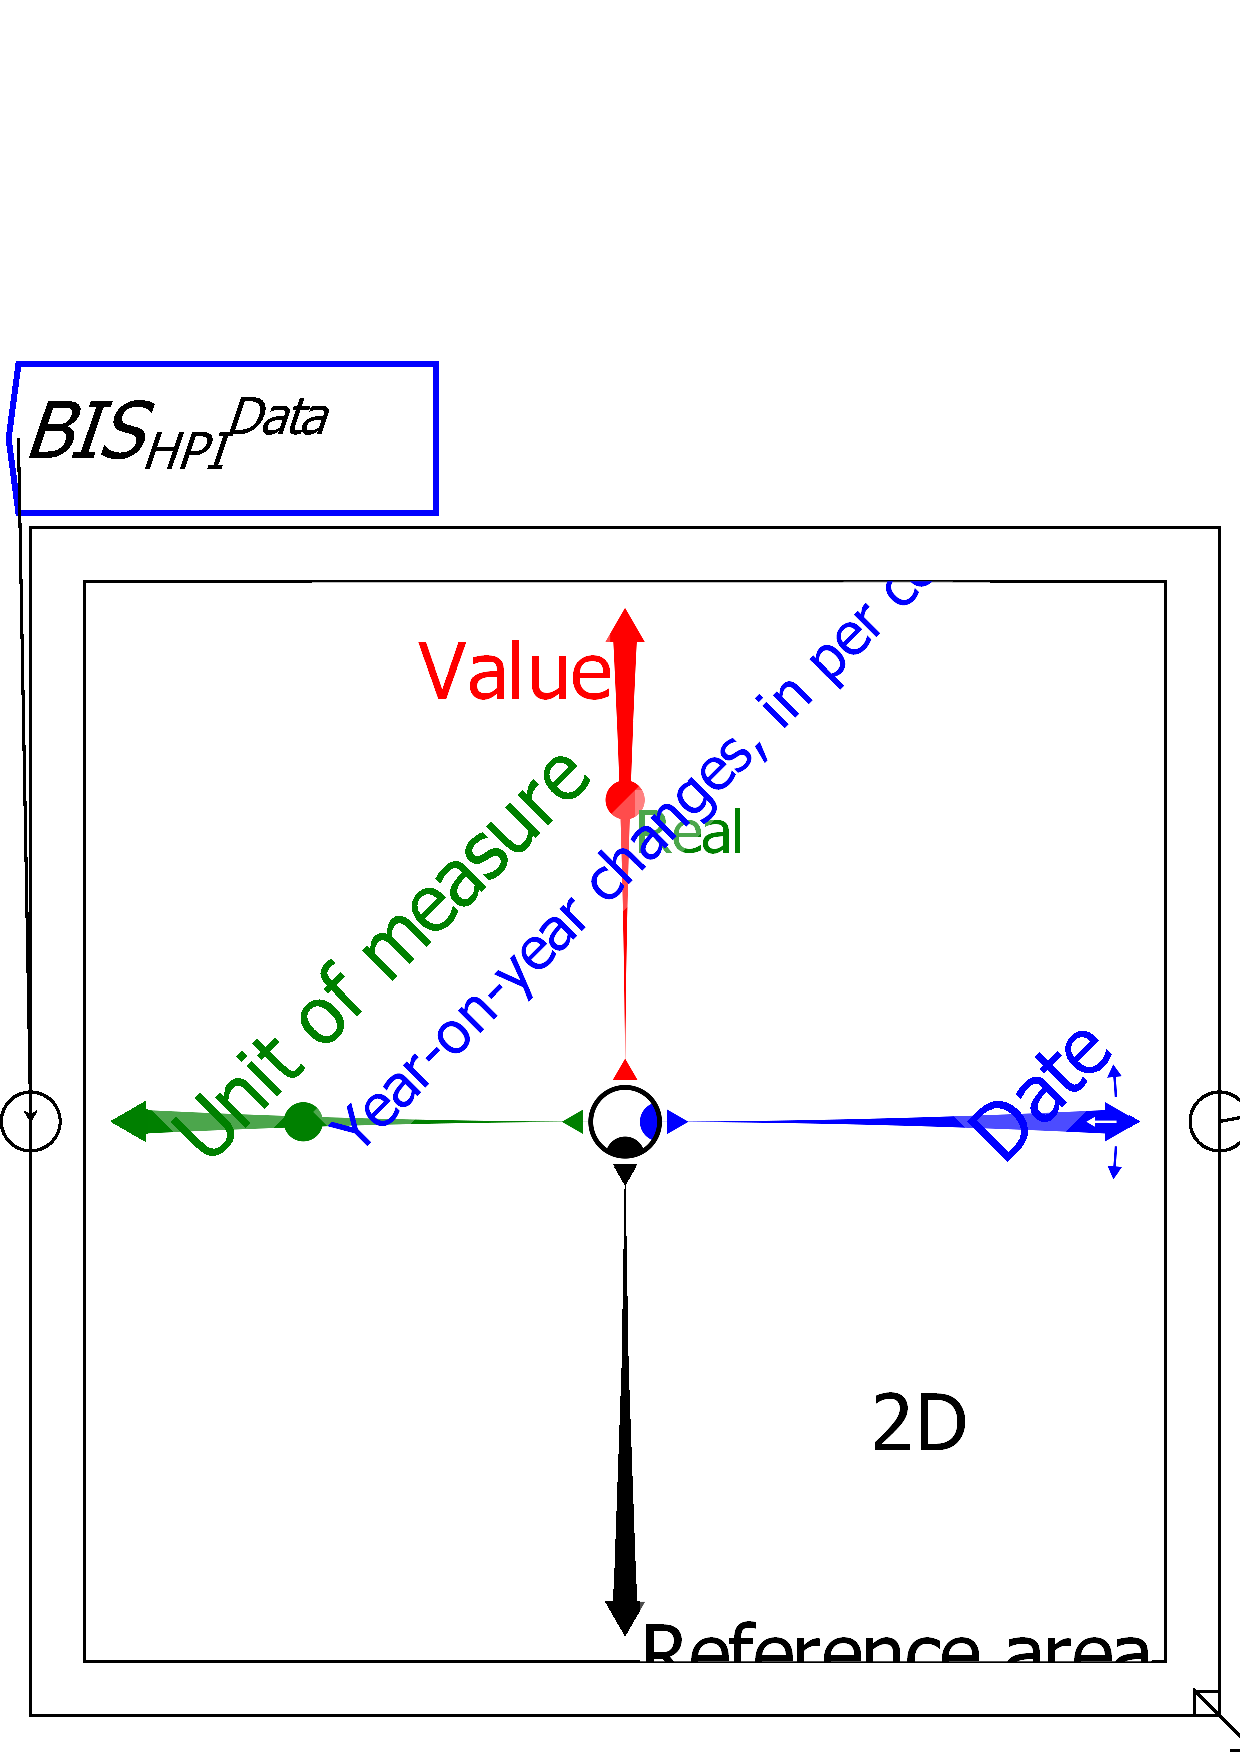
\includegraphics[width=\textwidth]{images/tut04HPI4DwithSheetRotatedCountryDateRealChange}

To really develop insights from your data, you attach the output of
the Ravel to variables, and analyse them using \emph{Ravel}'s flowchart
mathematics formulas.

\section{Attaching Variables to Ravels}

The source data file combines information on House Price Indices (where
the base year is 2010, so all indices are 100 during 2010), and the
annual rate of change of house prices, with data on both Nominal and
Real (CPI-deflated) prices. To analyse the data, it is useful to separate
it into House Price Index information and House Price Inflation information,
and to focus on Real rather than Nominal Prices. That is done by attaching
the output of the Ravel to Locks, and the Locks to named Variables
that you create.

The next image shows two variables $HPI_{Real}$ and $\Delta{HPI}$.
The lock for $\Delta{HPI}$ has been closed, while the lock for $HPI_{Real}$
is still open. Once the lock is closed, the output from that lock
remains the same, even if the selection on the source Ravel is altered.

\noindent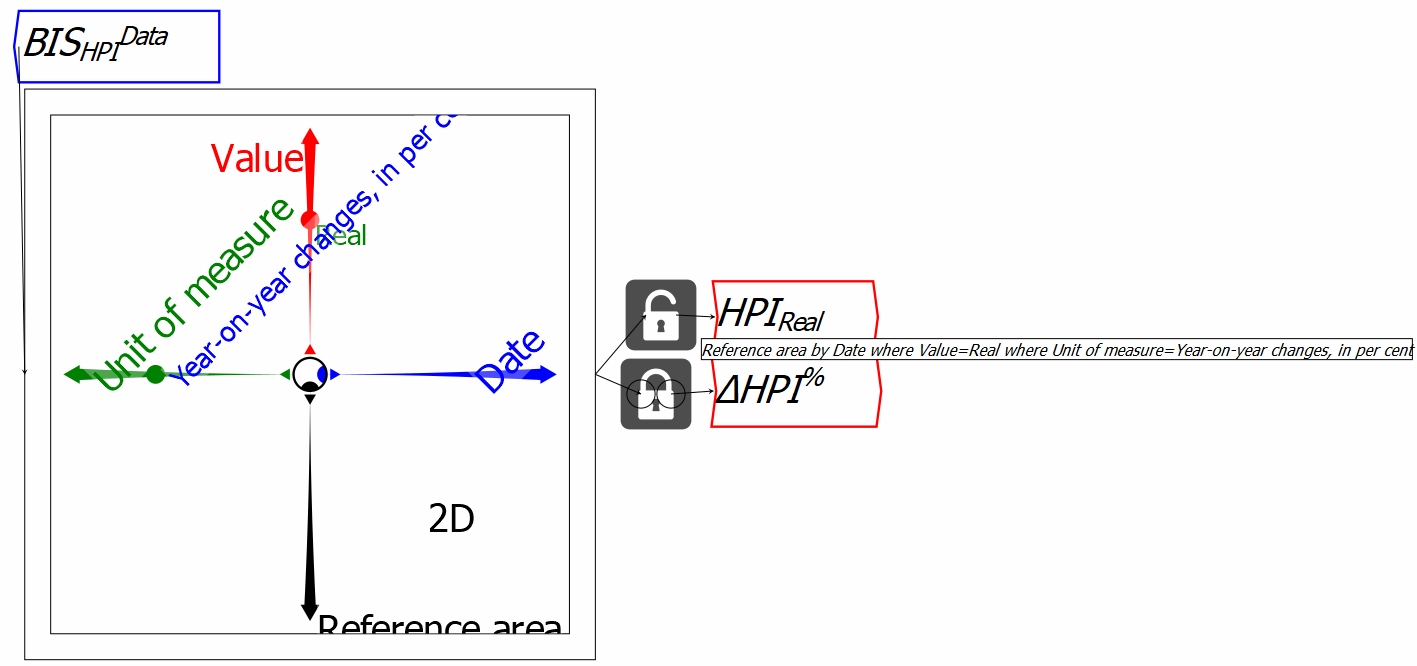
\includegraphics[width=\textwidth]{images/tut05HPIandInflationSeparatedLocks}

With the data separated into index and inflation data, we can now
focus on those subsets of the data rather than the entire source file.
The next image shows the source Ravel in icon mode, with the house
price inflation data attached to another Ravel and the currently selected
data displayed in a sheet.

\noindent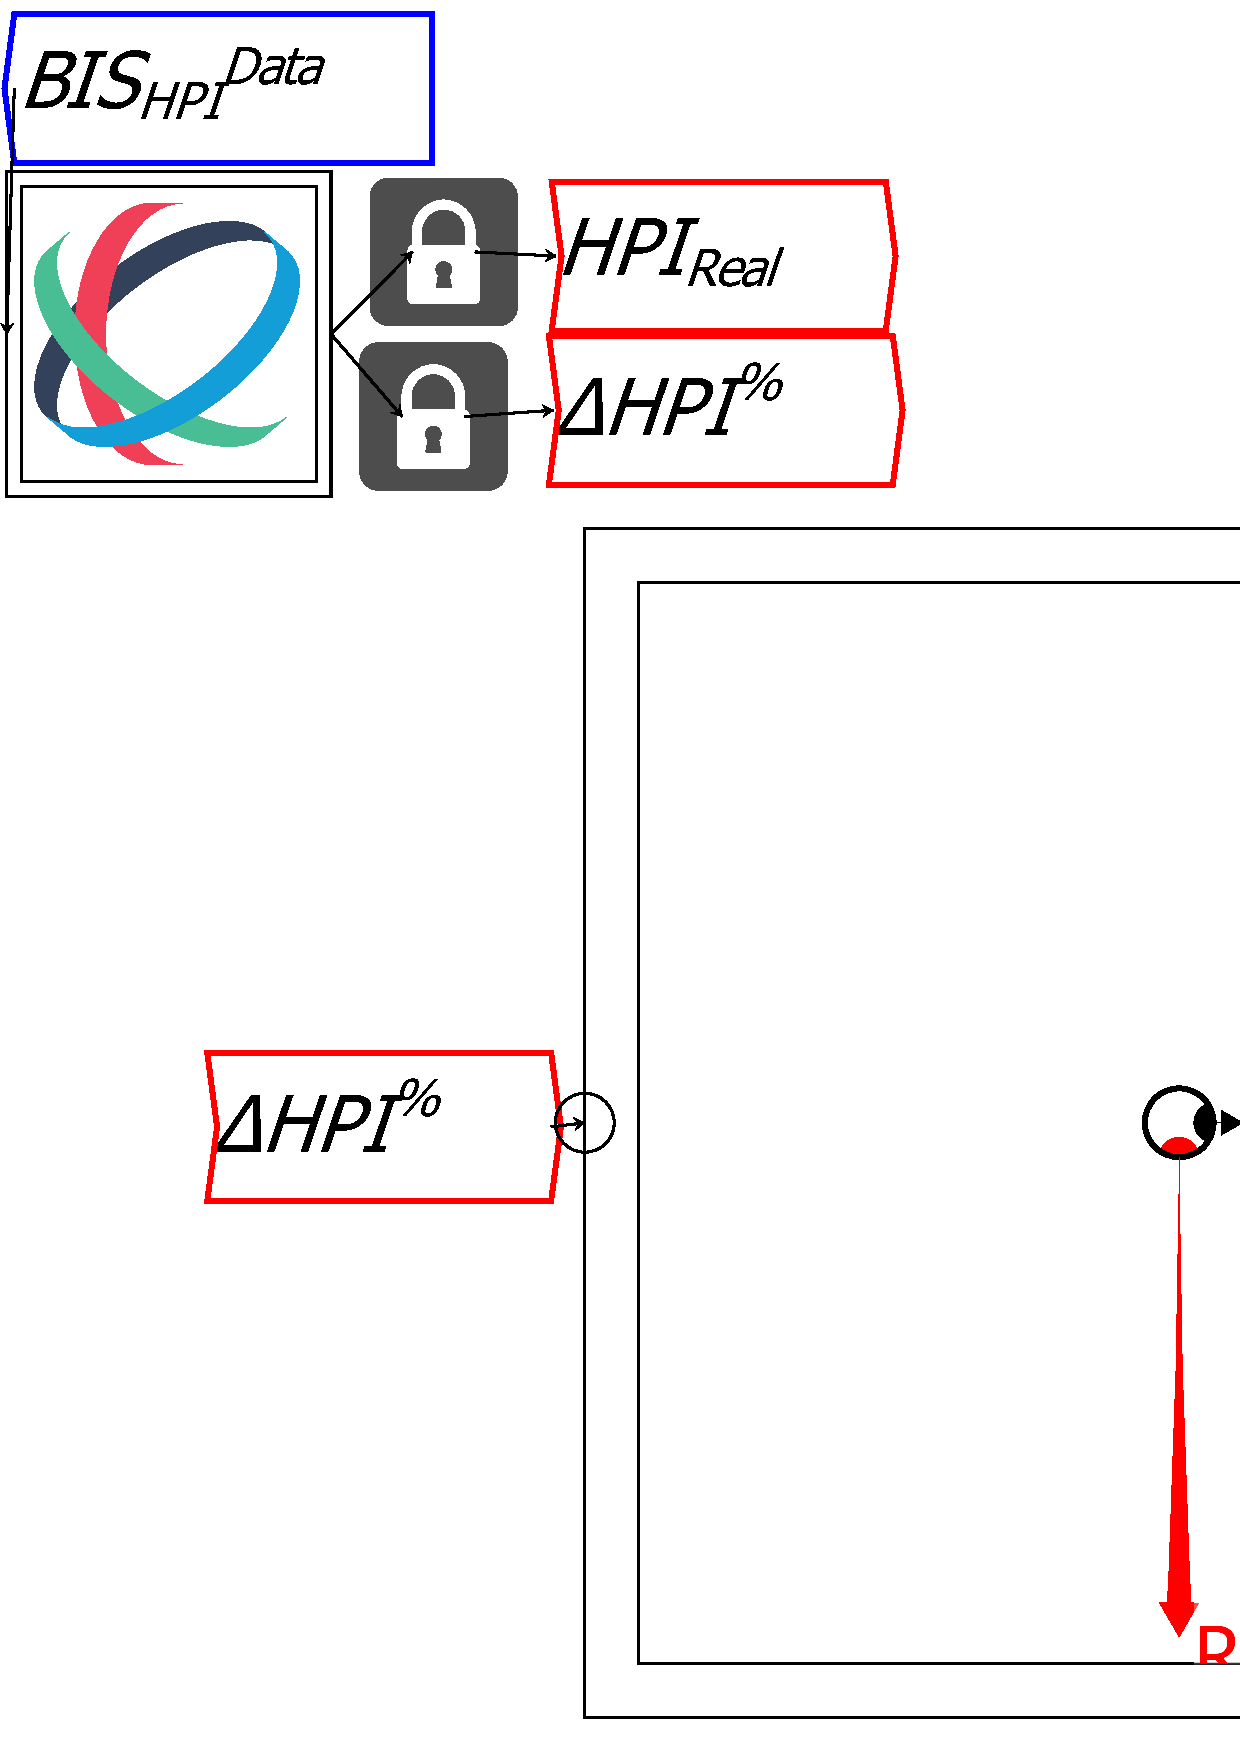
\includegraphics[width=\textwidth]{images/tut06HPIwithVariablesAssigned02DeltaHPI}

The information in the sheet suggests a possibly useful piece of analysis:
why not compare the average for all advanced countries (the first
entry on the Reference Area axis) to each advanced country?

The image below shows the result of attempting to do this by selecting
just the data for ``Advanced Economies'' using the selector dot, and
attaching that to a new variable $\Delta{HPI}_{Advanced}^{Avg}$,
while also selecting a number of advanced economies from the axis
(Australia, Austria, Belgium, etc.) and assigning that to another
variable $\Delta{HPI}_{Advanced}$.

\noindent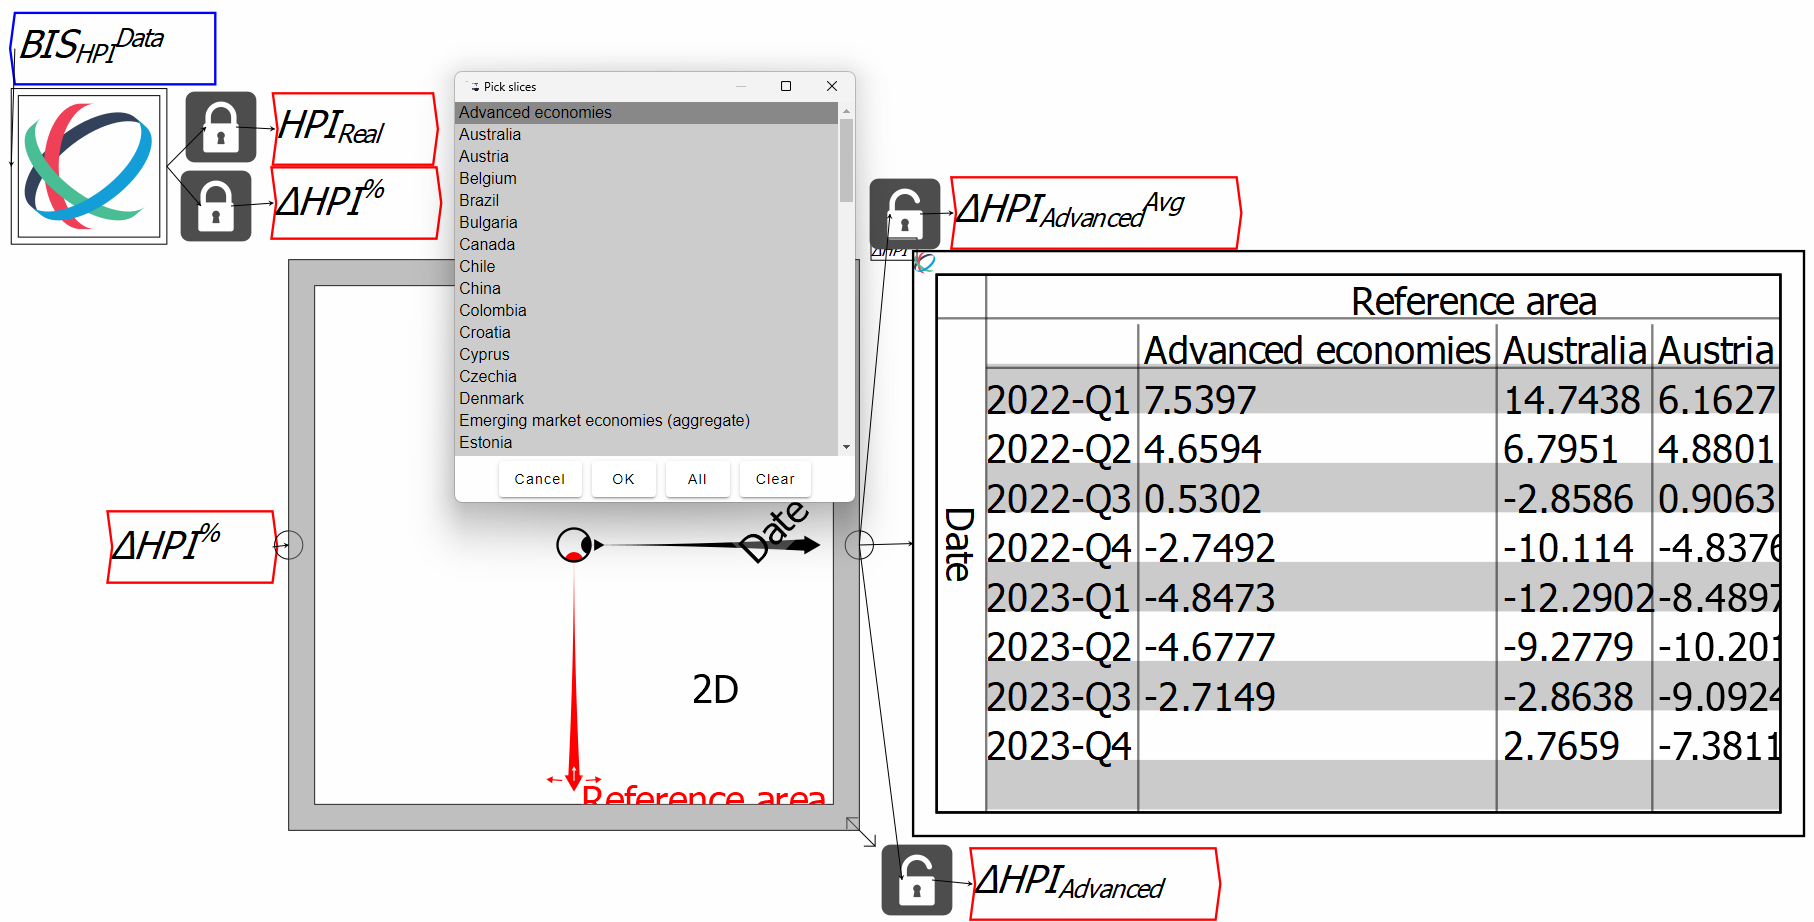
\includegraphics[width=\textwidth]{images/tut07SeparatingAdvancedAverage}

\section{Basic Analysis using \emph{Ravel}}

Data analysis can be done using the features of a Ravel alone. As
well as enabling the selection of display of different segments of
multidimensional data, you can perform basic data analysis by collapsing
the axes of a Ravel and applying various aggregations:
\begin{enumerate}
\item Summing an axis;
\item Multiplying axis elements by each other;
\item Extracting the maximum or minimum values along an axis; 
\item Calculating the average along an axis;
\item Calculating the standard deviation of an axis; and
\end{enumerate}
More advanced analysis can be performed by attaching the output of
a Ravel to a variable (preferably via a Lock \ref{Lock}, so that
the contents of the variable are unaffected by any subsequent manipulations
of the Ravel), and analysing it using \emph{Ravel}'s mathematical
operators. For more details see \ref{Operations}.

\section{Linking Ravels}

Ravels which have the same dimensions can be linked to each other.
For example, one Ravel may contain inflation data by country by month,
while another contains unemployment data by country by month. If the
two or more Ravels are linked, then selections applied to one Ravel
are applied to the other, which makes it easy to compare these variables
by country over time. For more details see \ref{Linking-Ravels}.

\section{Displaying your results in Sheets and Plots}

Ravels enable the selection and some analysis of data, but don't display
data themselves (however, we will embed Sheets and Plots into Ravels
in future releases of \emph{Ravel}). To see the output of a Ravel,
you need to attach the output of the Ravel (or variables derived from
it) to a Sheet or a Plot. For more details see \ref{Sheet} and \ref{PlotWidget}.

\section{Using Publication Tabs}

Calculations on the Wiring canvas can become too complicated for non-experts
to follow, so Publication tabs exist to enable you to show tailored
views of the results for different audiences---say one Tab for the
Marketing and another for the Accounting divisions of a company. For
details see \ref{tabs:Publication}.

\section{Working with Other Programs \label{Export}}

Though \emph{Ravel} can be used to present results very effectively,
you will sometimes wish to display your results in publication or
presentation software, or to create better-looking plots (Ravel's
Plots will improve dramatically in subsequent releases). You can export
a variety of formats from Ravel:
\begin{enumerate}
\item CSV files, in both columnar and tabular layout;
\item SVG, EPS and EMF vector and PNG bitmapped~graphics files, for use in word
processor and presentation software;
\item PDF format;
\item LaTeX format, for use in mathematical formatting programs like \LaTeX{}
editors and MathType; and
\item .m files, for analysis of the mathematics of a Ravel document in
  Matlab or Octave.
\end{enumerate}
Exporting is done in two main ways:
\begin{enumerate}
\item From the File menu option \emph{Export canvas as}, which exports an
entire canvas (this includes the Equations, Summary and Publication
Tabs)
\item From the context menu for any specific object, such as a Ravel, Variable,
Plot or Sheet.
\end{enumerate}

\section{Importing Data into Ravel}

CSV files typically have some columns that specify the nature
of data, while other columns contain the data itself. \emph{Ravel}
turns the fields specifying the nature of data into \emph{dimensions}
(which become axes of a Ravel), which enables the data to be manipulated
much more effectively than can be done with a spreadsheet. For data
to be imported into \emph{Ravel}, the dimensions must uniquely specify
each data point. This process is controlled by the import tool
\buttonIcon{importData}~, which then brings up the import
form in which you specify which columns to treat as dimensions and
which as data. For more details see \ref{CSV import} and \ref{Operation:csvImport}.
